\tikzstyle{block_a} = [rectangle, draw, %fill=blue!20,
     text width=2em, text centered, rounded corners, minimum height=3em]
\tikzstyle{block_b} = [rectangle, draw, %fill=blue!20,
     text width=7em, text centered, rounded corners, minimum height=5em]
\tikzstyle{line} = [draw, -latex]


\footnotesize

\begin{tikzpicture}[node distance = 2.5cm, every text node part/.style={align=center}]
    % Place nodes
    \node [] (input_image) at (0,0) {$I(j,k)$};
    \node [] (node1) at (1.5,0) {};

    \node [block_a, above right of=node1,  node distance=2cm] (gradiente_x) {$h_x$};
    \node [] () at (5,1.65){$G_x(j,k)=I(j,k)*h_x$};

    \node [block_a, below right of=node1, node distance=2cm] (gradiente_y) {$h_y$};
    \node [] () at (4.75,-1.7){$G_y(j,k)=I(j,k)*h_y$};
    %\node [] (node2) at (4,0) {};
    \node [block_b] (combinazione) at (6,0) {$G=\sqrt{G_x^2+G_y^2}$ \\ $\theta=atan\left(\tfrac{G_y}{G_x}\right)$};
    \node[right of = combinazione](uscita){$\mathbf{G}(j,k)$};

    % Draw edges
    \path [draw, -] (input_image) -- (node1);
    \path [line] (node1) |- (gradiente_x);
    \path [line] (node1) |- (gradiente_y);
    \path [line] (gradiente_x) -| (combinazione);
    \path [line] (gradiente_y) -| (combinazione);
     %\path [line] (node2) -- (combinazione);
     \path [line] (combinazione) -- (uscita);
\end{tikzpicture}
